\appendix

\section{Proofs for Section 3}

\subsection{Proof of Theorem \ref{theorem:LT-Convexity}}
\label{proof:convexity}

To prove Theorem~\ref{theorem:LT-Convexity}, we first show that the
real-time objective is jointly convex with respect to
$(\Vector{q}^l,\Vector{m},\Vector{\lambda}).$
\begin{lemma}
	\label{lemma:rt-convex}
	$\tilde{F}^r$ as defined in \eqref{eq:rt-obj2} is jointly
        convex with respect to
        $(\Vector{q}^l,\Vector{m},\Vector{\lambda})$ over
        $\mathbb{R}^N_+ \times C(L^r).$
\end{lemma}
\begin{proof}
	We rewrite
	\begin{eqnarray}
          \tilde{F}^r(\Vector{q}^l,\Vector{m},\Vector{\lambda},\Vector{p}^r,\Vector{w}^r) = \sum_{i=1}^{N} p^l_i [m_i-w^r_i-q^l_i]_+ \nonumber \\
          + \beta \sum_{i=1}^{N} \frac{\lambda_i}{\mu_i - \lambda_i/m_i} + \beta \sum_{i=1}^{N}\sum_{j=1}^{J} \lambda_{ji} \pi_{ij}.
	\end{eqnarray}
	
        %	$\sum_{i=1}^{N} p^l_i q^l_i$ and
        % $\sum_{i=1}^{N}\sum_{j=1}^{J} \lambda_{ji} \pi_{ij}$ are
        % convex.
	
	Since $m_i-w^r_i-q^l_i$ is an affine function, and $[\cdot]_+$
        is convex and non-decreasing, $\sum_{i=1}^{N} p^l_i
        [m_i-w^r_i-q^l_i]_+$ is jointly convex with respect to
        $(\Vector{q}^l,\Vector{m}).$
	
	Here, we need to show that
        $\sum_{i=1}^{N}\frac{\lambda_i}{\mu_i - \lambda_i/m_i}$ is
        jointly convex with respect to $(m_i,\lambda_i).$ We have
        $\frac{\bar{\lambda}_i}{\mu_i - \bar{\lambda}_i}$ is
        non-decreasing and convex in $0 \leq \bar{\lambda}_i \leq
        \mu_i$, and $\bar{\lambda}_i=\lambda_i/m_i$ is convex over
        $\lambda_i \geq 0$ and $m_i \geq 0$. So,
        $\frac{\lambda_i/m_i}{\mu_i - \lambda_i/m_i}$ is convex. In
        addition, $m_i$ is non-negative so $\frac{\lambda_i}{\mu_i -
          \lambda_i/m_i}$ is convex because the perspective of a
        convex function is convex \cite{boyd2004convex}).
	
	Since $\lambda_i = \sum_{j}^{} \lambda_{ij}$ is linear and
        non-decreasing, $\frac{\sum_{j}^{} \lambda_{ij}}{\mu_i -
          (\sum_{j}^{} \lambda_{ij})/m_i}$ is convex. Thus,
        $\tilde{F}^r$ is jointly convex with respect to
        $(\Vector{q}^l,\Vector{m},\Vector{\lambda})$ because the
        summation of convex functions are convex.
\end{proof}

\begin{proof}[of Theorem~\ref{theorem:LT-Convexity}]
  From Lemma~\ref{lemma:rt-convex}, we know that the real time
  objective function
  $\tilde{F}^r(\Vector{q}^l,\Vector{m},\Vector{\lambda},\Vector{p}^r,\Vector{w}^r)$
  is jointly convex with respect to
  $(\Vector{q}^l,\Vector{m},\Vector{\lambda}).$ It then follows
  that $$F^{*r}(\Vector{q}^l,\Vector{p}^r, \Vector{L}^r, \Vector{w}^r)
  = \min_{(\Vector{m},\Vector{\lambda}) \in C(L^r)}
  \tilde{F}^r(\Vector{q}^l,\Vector{m},\Vector{\lambda},\Vector{p}^r,\Vector{w}^r)$$
  is convex with respect to $\Vector{q}^l$ (see
  \cite{boyd2004convex}). Finally, since the expectation operation
  preserves convexity, we conclude that $F^l(\Vector{q}^l)$ is convex
  with respect to $\Vector{q}^l.$
\end{proof}


\subsection{Proof of Theorem~\ref{theorem:lt_gradient}}
\label{proof:lt_grad}

This section is devoted to the proof of
Theorem~\ref{theorem:lt_gradient}.  \ignore{Let us
  define $$F^{*r}(q^l,p^r,L^r,w^r):= \min_{(m,\Lambda) \in C(L^r)}
  F^r(q^l,m,\Lambda,p^r,w^r).$$ With this notation, note
  that $$\hat{F}^l(q^l,p^r,L^r,w^r) = \sum_{i \in N} p^l_i q^l_i +
  F^{*r}(q^l,p^r,L^r,w^r).$$} To prove
Theorem~\ref{theorem:lt_gradient}, it suffices to show that
\begin{equation}
  \label{eq:lt_gradient_1}
  \begin{array}{rl}
    \frac{\partial \Exp{F^{*r}(\Vector{q}^l,\Vector{p}^r,\Vector{L}^r,\Vector{w}^r)}}{\partial q^l_i} &= \Exp{\frac{\partial F^{*r}(\Vector{q}^l,\Vector{p}^r,\Vector{L}^r,\Vector{w}^r)}{\partial q^l_i}}\\
  &=
  -\Exp{\varrho_i(\Vector{q}^l,\Vector{p}^r,\Vector{L}^r,\Vector{w}^r)}.      
  \end{array}
\end{equation}
The first step is to prove that the Lagrange multiplier of GLB-RT
corresponding to the constraint \eqref{eq:GLB-RT_c3} is unique.
\ignore{
\jk{Add assumption earlier that wind follows a continuous
  distribution. We need this for the following reason: The proof of
  uniqueness of the Lagrange multiplier requires that the constraint
  $m_i \geq 0$ is not binding. This becomes problematic when the
  optimal $\lambda_i = 0,$ in which case the optimal $m_i$ becomes
  ill-posed. One (not very elegant) fix to this is to assume $w^r$ is
  continuous. This implies that $w^r_i > 0$ with probability 1, which
  implies that we may take $m_i> 0$ with probability 1.}}
\begin{lemma}
  \label{lemma:lt_grad_1}
  With probability 1, GLB-RT has a unique Lagrange multiplier, denoted
  $\varrho_i(\Vector{q}^l,\Vector{p}^r,\Vector{L}^r,\Vector{w}^r),$
  corresponding to the constraint \eqref{eq:GLB-RT_c3}.
\end{lemma}
\begin{proof}
  In this proof, for notational simplicity, we suppress the dependence
  of the primal and dual solutions of GLB-RT on
  $(\Vector{q}^l,\Vector{p}^r,\Vector{L}^r,\Vector{w}^r).$ Consider a
  primal solution of GLB-RT
  $(\Vector{q}^r,\Vector{m},\Vector{\lambda})$ with $\Vector{m} > 0.$
  Such a solution exists with probability 1, since $\Vector{w}^r > 0$
  with probability 1.

  Now any dual solution must satisfy the KKT conditions. This implies
  the following conditions. (Since the constraint $\lambda_i \leq m_i
  \mu_i$ is never binding, the corresponding Lagrange multiplier
  $\sigma_i = 0$ and does not feature in the following.)
\begin{align}
  \label{eq:kkt_1}
  &- \beta \bigg (\frac{\frac{\lambda_i}{m_i}}{\mu_i - \frac{\lambda_i}{m_i}}\bigg)^2 + \bar{\omega}_i - \underbar{$\omega$}_i + \varrho_i = 0 \\
  \label{eq:kkt_2}
  &\bar{\omega}_i(m_i - M_i) = 0; \bar{\omega}_i \geq 0, m_i \leq M_i \\
  \label{eq:kkt_3}
  &\underbar{$\omega$}_i m_i = 0; \underbar{$\omega$}_i \geq 0, m_i \geq 0 \\
  \label{eq:kkt_4}
  &p_i^r - \kappa_i - \varrho_i = 0 \\
  \label{eq:kkt_5}
  &\kappa_i q^r_i = 0; \kappa_i \geq 0, q^r_i \geq 0 \\
  \label{eq:kkt_6}
  &\varrho_i(-q^r_i + m_i - w^r_i - q^l_i)  = 0; \\
  \label{eq:kkt_7}
  &\varrho_i \geq 0, q^r_i \geq m_i - w^r_i - q^l_i
\end{align}

We now argue that $\varrho_i$ is unique for all $i.$ Consider the
following two cases.

\noindent {\bf Case 1:} $w^r_i + q^l_i > M_i.$ In this case, it
follows that $m_i <w^r_i + q^l_i + q^r_i.$ Using \eqref{eq:kkt_6}, we
conclude that $\varrho_i = 0.$

\noindent {\bf Case 2:} $w^r_i + q^l_i < M_i.$ Here we consider two
sub-cases. \\
{\bf Case 2a:} $m_i = M_i.$ In this case, it follows that $q^r_i > 0,$
which implies that $\kappa_i = 0$ (by \eqref{eq:kkt_5}). Thus, we
have, using \eqref{eq:kkt_4}, that $\varrho_i = p^r_i.$\\
{\bf Case 2b:} $m_i < M_i.$ In this case, since $m_i \in (0,M_i),$ we
have $\bar{\omega}_i = \underbar{$\omega$}_i = 0$ 
(by \eqref{eq:kkt_2}
and \eqref{eq:kkt_3}). Thus, from \eqref{eq:kkt_1}, we
have $$\varrho_i = \beta \bigg (\frac{\frac{\lambda_i}{m_i}}{\mu_i -
  \frac{\lambda_i}{m_i}}\bigg)^2.$$

Since the event $w^r_i + q^l_i = M_i$ has zero probability, we may
ignore this case. This completes the proof.
%The idea is that if the Lagrange multiplier $\varrho_i(\Vector{q}^l,\Vector{p}^r,\Vector{L}^r,\Vector{w}^r)$ is not unique, it cannot be obtained by optimizing GLB-RT.
%
%Assuming that $\frac{\partial F^{*r}(q^l,p^r,L^r,w^r)}{\partial q^l_i} = \varrho_i(\Vector{q}^l,\Vector{p}^r,\Vector{L}^r,\Vector{w}^r)$ is not unique, there exist two optimal solutions $\underline{q}^{l}_i$ and $\bar{q}^l_i$ at data center $i$ such that 
%$$\frac{\partial \Exp{F^{*r}(.)}}{\partial \underline{q}^{l}_i} \neq \frac{\partial \Exp{F^{*r}(.)}}{\partial \bar{q}^{l}_i} $$
%
%Since $F^{*r}(.)$ is convex over $q^l_i$, we have ${q}^{\gamma}_i = \chi \underline{q}^{l}_i + (1-\gamma) \bar{q}^{l}_i$ with $0<\gamma<1$ such that
%$F^{*r}({q}^{\gamma}_i) \leq F^{*r}(\bar{q}^{l}_i) + (1-\gamma)F^{*r}(\underline{q}^{l}_i)$. 
%$F^{*r}(\bar{q}^{l}_i)$ and $F^{*r}(\bar{q}^{l}_i)$ are both optimal, thus  
%$$F^{*r}({q}^{\gamma}_i) = F^{*r}(\bar{q}^{l}_i) + (1-\gamma)F^{*r}(\underline{q}^{l}_i)$$ which means that $F^{*r}$ is linear on $[\underline{q}^{l}_i, \bar{q}^l_i]$. Hence, its gradients on $[\underline{q}^{l}_i, \bar{q}^l_i]$ are constant that contradicts the assumption.
\end{proof}

Given Lemma~\ref{lemma:lt_grad_1}, it follows from standard
sensitivity analysis in convex optimization (see Section~6.5.3 and
~6.5.4 in \cite{Bertsekas03}) that 
\begin{equation}
  \label{eq:grad_lt}
  \frac{\partial
    F^{*r}(\Vector{q}^l,\Vector{p}^r,\Vector{L}^r,\Vector{w}^r)}
  {\partial q^l_i} =-
  \varrho_i(\Vector{q}^l,\Vector{p}^r,\Vector{L}^r,\Vector{w}^r).  
\end{equation}
This proves the second equality in \eqref{eq:lt_gradient_1}. Thus, to
complete the proof of Theorem~\ref{theorem:lt_gradient}, it only
remains to justify the interchange of the partial derivative and the
expectation in the first equality. We justify this interchange by
invoking the dominated convergence theorem as follows.

Let $e_i$ denote a column vector in $\mathbb{R}^N,$ with 1 in the
$i$th entry and 0 elsewhere.
\begin{lemma}
  \label{lemma:lt_grad_2}
  For any $\delta \neq 0$ and $i \in N,$
  \begin{equation*}
    \left|\frac{F^{*r}(\Vector{q}^l + \delta e_i,\Vector{p}^r,\Vector{L}^r,\Vector{w}^r) - 
        F^{*r}(\Vector{q}^l,\Vector{p}^r,\Vector{L}^r,\Vector{w}^r)}{\delta}\right| \leq p^r_i.
  \end{equation*}  
\end{lemma}
\begin{proof}
  It is easy to see
  that $$F^{*r}(\Vector{q}^l,\Vector{p}^r,\Vector{L}^r,\Vector{w}^r)
  \leq \delta p^r_i + F^{*r}(\Vector{q}^l + \delta
  e_i,\Vector{p}^r,\Vector{L}^r,\Vector{w}^r).$$ The statement of
  Lemma~\ref{lemma:lt_grad_2} follows from the fact that
  the function $F^{*r}(\Vector{q}^l + \delta
  e_i,\Vector{p}^r,\Vector{L}^r,\Vector{w}^r)$ is non-increasing with
  respect to $\delta.$
\end{proof}

Since $\Exp{p^r_i} < \infty,$ it follows from the dominated
convergence theorem that 
\begin{align*}
  &\Exp{\lim_{\delta \ra 0} \frac{F^{*r}(\Vector{q}^l + \delta
      e_i,\Vector{p}^r,\Vector{L}^r,\Vector{w}^r) -
      F^{*r}(\Vector{q}^l,\Vector{p}^r,\Vector{L}^r,\Vector{w}^r)}{\delta}} \\
  &\quad =\lim_{\delta \ra 0} \frac{\Exp{F^{*r}(\Vector{q}^l + \delta
      e_i,\Vector{p}^r,\Vector{L}^r,\Vector{w}^r)} -
    \Exp{F^{*r}(\Vector{q}^l,\Vector{p}^r,\Vector{L}^r,\Vector{w}^r)}}{\delta}.
\end{align*}
This proves the first equality in \eqref{eq:lt_gradient_1}, and
completes the proof of the theorem.


\subsection{Proof of Lemma~\ref{theorem:RealTimeOptimalDemand}}
\label{proof:RealTimeOptimalDemand}

 We assume there an optimal solution $S$ such that $\lambda_i>0$ and $0 < m_i < w^r_i + q^l_i$. $\lambda_i=0$ or $m_i = 0$ is not ignored because it is equivalent to shutting down data center $i$. Here, $\underbar{$\omega$}_i=\varrho_i = 0$.
 
 If $w^r_i + q^l_i < M_i$ and $m_i < w^r_i + q^l_i$, $\bar{\omega}_i = 0$. $\bar{\omega}_i = \underbar{$\omega$}_i=\varrho_i = 0$ results in $\lambda_i/m_i$ becomes zero as \eqref{eq:kkt_1}. $\lambda_i=0$ or $m_i = \infty$ contradicts the assumption. So, $m_i \geq w^r_i+q^l_i$ if $w^r_i + q^l_i < M_i$. 
 
 If $w^r_i + q^l_i \geq M_i$, we assume that $m_i < M_i$. $\bar{\omega}_i = \underbar{$\omega$}_i=\varrho_i = 0$ again leads to the contradiction to the assumption. So, $m_i=M_i$ if $w^r_i + q^l_i \geq M_i$.

\section{Convergence of SGA}
\label{sec:conv-proof}

This section is devoted to the proof of Theorem~\ref{thm:sgea}.
Invoking Theorem~2.1 in \cite{Kushner03}, the almost sure convergence
of the iterates of SGA to the set of optimal solutions of EP-LT holds
if the following two conditions are satisfied.
  \begin{enumerate}
  \item $\nabla F^l:\R^N_+ \ra \R^N$ is continuous.
  \item $ \sup_{q^l \in \R^N_+}
    \Exp{(\varrho_i(\Vector{q}^l,\Vector{p}^r,\Vector{L}^r,\Vector{w}^r))^2}
    < \infty.$
  \end{enumerate}
  Condition~(1) above holds since the gradient of a differentiable
  convex function is convex; see Theorem 25.5 in
  \cite{Rockafellar70}. Condition~(2) holds since $$
  \varrho_i(\Vector{q}^l,\Vector{p}^r,\Vector{L}^r,\Vector{w}^r) \leq
  p^r_i$$ (see \eqref{eq:grad_lt} and
  Lemma~\ref{lemma:lt_grad_2}). This completes the proof.



% \begin{lemma}
%   \label{lemma:sgea-3}
%   The iterates $q^l(n)$ generated by the SGEA algorithm are almost
%   surely bounded.
% \end{lemma}
% \jk{This is also easy. If any component $i$ of $q^l_i$ exceeds
% $M_i$, then
% $\varrho_i(\Vector{q}^l,\Vector{p}^r,\Vector{L}^r,\Vector{w}^r) = 0$
% for any $(\Vector{p}^r,\Vector{L}^r,\Vector{w}^r),$ implying the
% algorithm will necessarily decrease $q^l_i.$}

%\section{Figures for predictability analysis}
%
%\subsection{Electricity prices}
%
%\begin{figure}[!t]
%	\centering
%	\subfloat[Houton, Texas]{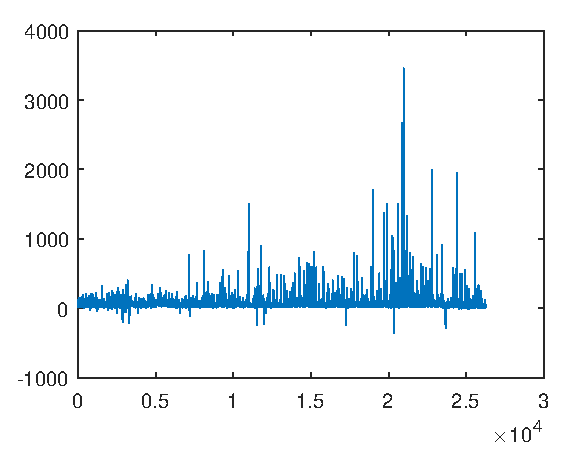
\includegraphics[width=.5\linewidth]{figs2/electricity_prices_TX}}
%	\subfloat[Ohio]{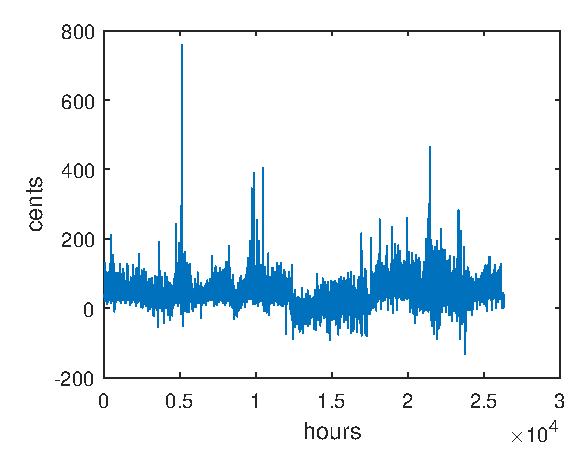
\includegraphics[width=.5\linewidth]{figs2/electricity_prices_OH}}
%	\caption{Electricity prices.}
%	\label{fig:electricityPrices}
%\end{figure}

